\chapter{Implementation}
\label{cha:Implementation}

\section{Generalising the Codebase}
\label{sec:Generalising the Codebase}
The first step in development was to modify the AIM4 codebase so that it could be more easily adapted to work with other simulations. This ended up being a more difficult task than expected and much of the code has been refactored out into general and AIM specific classes, in order to allow it to be extended effectively. There are still some artefacts left over in the generalised code from AIM, however the vast majority has been removed. 

Generalising the codebase was done in conjunction with Rebecca Milligan, who is also working on AV simulations in her car park management project.

\subsection{aim4.driver}
\label{subsec:aim4.driver}
Figure \ref{fig:driverBefore} is a class diagram indicating the structure of Driver and it's subclasses before changes were made. Figure \ref{fig:driverAfter} shows the structure in the generalised codebase.

\begin{figure}[htb]
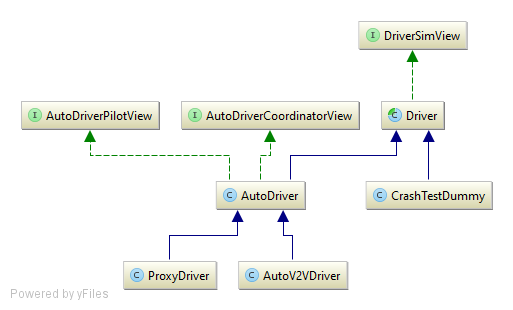
\includegraphics[width=\textwidth]{class_diagrams/driverBefore.png}
\caption{Original class structure for aim4.driver.}
\label{fig:driverBefore}
\end{figure}

\begin{figure}[htb]
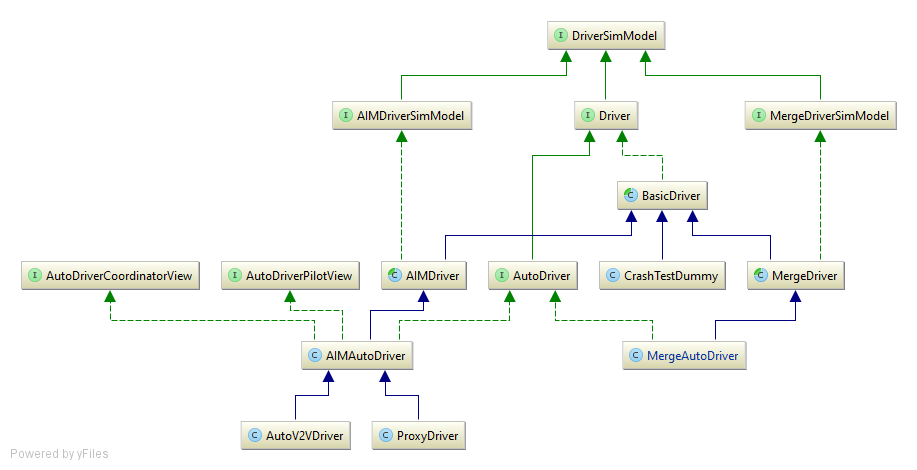
\includegraphics[width=\textwidth]{class_diagrams/driverAfter.png}
\caption{New class structure for aim4.driver, after changes were made generalising the codebase.}
\label{fig:driverAfter}
\end{figure}

The first major change was renaming \emph{DriverSimView}, \emph{AutoDriverPilotView}, and \emph{AutoDriverCoordinatorView} to end in \emph{Model} instead of \emph{View}. These interfaces are used to limit the methods that other classes can access in Driver and AutoDriver, thus changing their 'view' of that class. We didn't want to continue using \emph{View} as it could cause confusion with the GUI elements of the simulator. \revisit{We chose to refer to these interfaces as \emph{Models}, because the accessors are effectively given a model of Driver and AutoDriver (beyond which they care very little) that they can use to access the methods they want.}

The next change was separating out all of the AIM specific code into its own classes and interfaces. You can see how this was done in Figure \ref{fig:driverAfter} with \emph{AIMDriverSimModel} and \emph{AIMDriver}. By extracting AIM specific behaviour, we created general classes that could be extended, reducing code duplication. The merge specific code found in \emph{MergeDriverSimModel}, \emph{MergeDriver} and \emph{MergeAutoDriver} is structured in a very similar manner to its AIM counterpart, taking advantage of the generalised code. However, as a consequence of breaking out the code like this, a number of additional changes had to be made. 

\revisit{Driver was broken out into an interface and a new class \emph{BasicDriver}. Driver is simply used as an interface for accessing Drivers in non-simulation contexts (such as \emph{BasicVehicle}). \emph{BasicDriver} contains the generalised functionality all \emph{Driver} should need, with AIM specific activities moved to \emph{AIMDriver}. Extending from \emph{Driver} is the \emph{AutoDriver} interface, which adds no new methods but is instead used to categorise autonomous drivers. \emph{AIMAutoDriver} contains almost exactly the same code as the original \emph{AutoDriver} class.}

\subsection{aim4.gui}
\label{subsec:aim4.gui}
In the original simulator, shown in Figure \ref{fig:originalAIMSetupLabeled} \emph{Viewer.mainPanel} displays the simulator setup and canvas using a \emph{CardLayout}. In the new GUI, shown in Figure \ref{fig:newAIMSetupLabeled} we replaced \emph{mainPanel} with \emph{tabbedPane}, a \emph{JTabbedPane} object that allows users to switch between different simulators. On each tab we added a \emph{SimViewer} object, shown in Figure \ref{fig:simViewer}, which behaves in the same way that \emph{mainPanel} did in the original code. Each \emph{SimViewer} has two panels, a \emph{SimSetupPanel} and a \emph{SimScreen}, which it can switch between using \emph{CardLayout}. Functionality from \emph{SimSetupPanel} was extracted out into AIM specific and general classes. It is used to create and modify \emph{SimSetup} objects. \emph{SimScreen} is a new interface which \emph{Canvas} inherits from. It is used to allow \emph{SimViewer} to display screens other than \emph{Canvas} such as \emph{MergeStatScreen}. You can see how \emph{SimSetupPanel} and \emph{SimScreen} are structured in Figures \ref{fig:simSetupPanel} and \ref{fig:simScreen}.

\begin{figure}[htb]
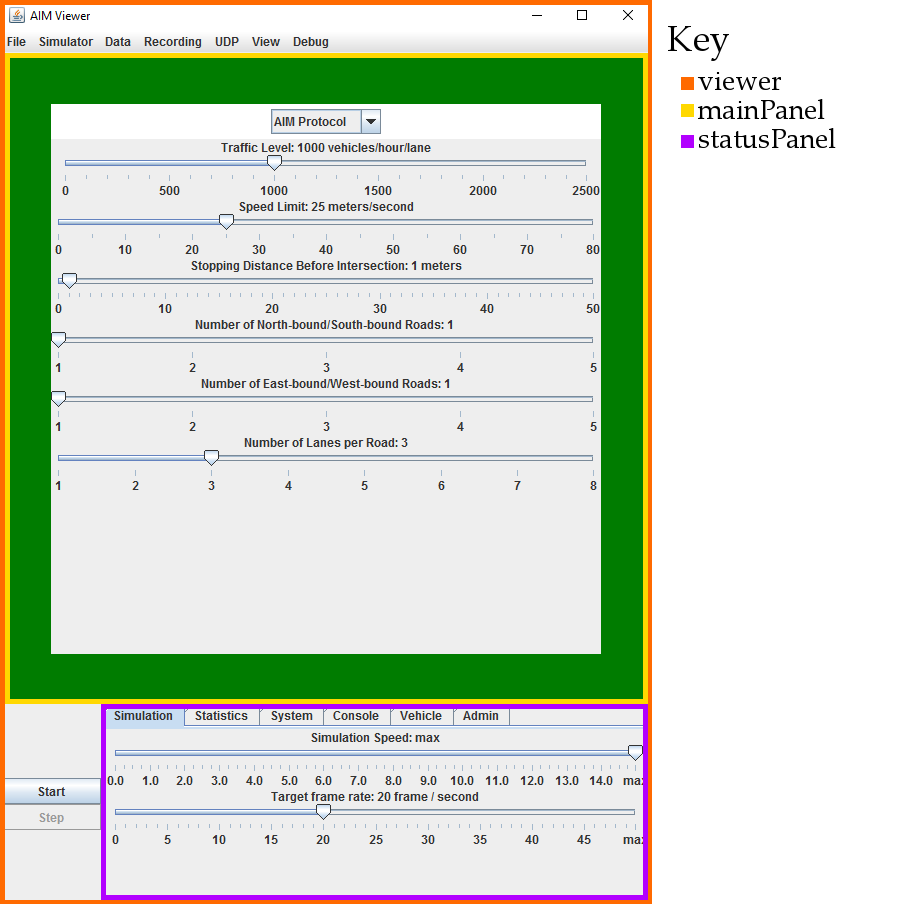
\includegraphics[width=\textwidth]{screenshots/originalAIMSetupLabeled.png}
\caption{Panel layout in the original Viewer}
\label{fig:originalAIMSetupLabeled}
\end{figure}

\begin{figure}[htb]
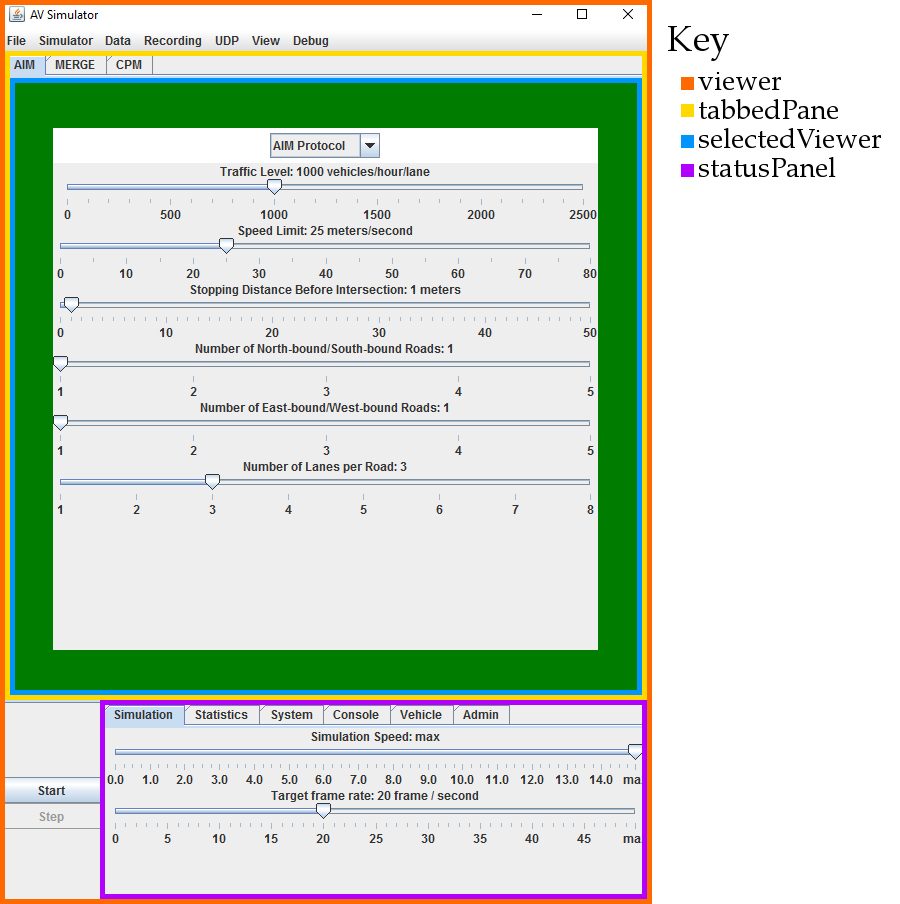
\includegraphics[width=\textwidth]{screenshots/newAIMSetupLabeled.png}
\caption{Panel layout in the new Viewer}
\label{fig:newAIMSetupLabeled}
\end{figure}

\begin{figure}[htb]
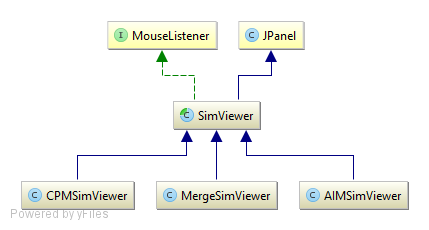
\includegraphics[width=\textwidth]{class_diagrams/simViewer.png}
\caption{The class diagram for SimViewer}
\label{fig:simViewer}
\end{figure}

\begin{figure}[htb]
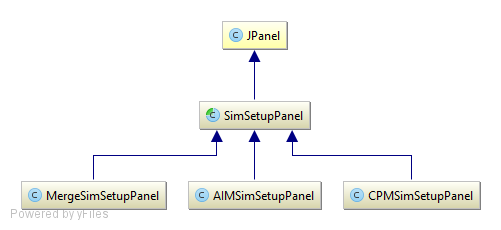
\includegraphics[width=\textwidth]{class_diagrams/simSetupPanel.png}
\caption{The class diagram for SimSetupPanel}
\label{fig:simSetupPanel}
\end{figure}

\begin{figure}[htb]
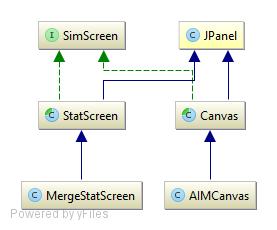
\includegraphics[width=\textwidth]{class_diagrams/simScreen.png}
\caption{The class diagram for SimScreen}
\label{fig:simScreen}
\end{figure}

We also made a small adjustment to the behaviour of the reset option in the menu. The simulator must be paused in order for the reset button not to be greyed out.

\subsection{aim4.map}
\label{subsec:aim4.map}
Map had a few structure changes made in order to allow for maps without grid based intersections. You can see how the changes were made in Figures \ref{fig:mapBefore} and \ref{fig:mapAfter}. 

\begin{figure}[htb]
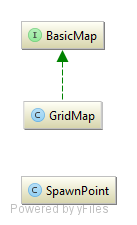
\includegraphics[width=\textwidth]{class_diagrams/mapBefore.png}
\caption{The original class structure for BasicMap and SpawnPoint.}
\label{fig:mapBefore}
\end{figure}

\begin{figure}[htb]
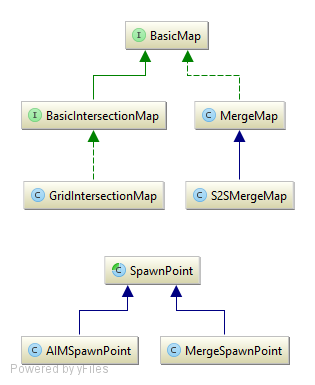
\includegraphics[width=\textwidth]{class_diagrams/mapAfter.png}
\caption{The new class structure for BasicMap and SpawnPoint.}
\label{fig:mapAfter}
\end{figure}

One of the major changes was breaking out \emph{SpawnPoint} into general and AIM specific features. This had to be done because \emph{SpawnPoint} was creating \emph{SpawnSpec} objects with \emph{destination} fields. \emph{destination} is an AIM specific field relating to the intersection exit a vehicle plans to reach.

